\hypertarget{markov-chain-monte-carlo}{%
\section{Markov Chain Monte Carlo}\label{markov-chain-monte-carlo}}

\hypertarget{sampling}{%
\subsection{Sampling}\label{sampling}}

Markov Chain Monte Carlo (MCMC) is a useful method whenever we have a probability distribution that we want to sample from but there is not direct sampling way to do so.

In almost any computer simulation the ultimate source of randomness is a stream of (close to) uniform, uncorrelated bits generated from a pseudo random number generator. A direct sampling method takes such a source and outputs uncorrelated samples from the target distribution. The fact they're uncorrelated is key as we'll see later. Examples of direct sampling methods range from the trivial: take n random bits to generate integers uniformly between 0 and \(2^n\) to more complex methods such as inverse transform sampling and rejection sampling \autocite{devroyeRandomSampling1986}.

In physics the distribution we usually want to sample from is the Boltzmann probability over states of the system \(S\): \[
\begin{aligned}
p(S)  &= \frac{1}{\mathcal{Z}} e^{-\beta H(S)} \\
\end{aligned}
\] where \(\mathcal{Z} = \sum_S e^{-\beta H(S)}\) is the normalisation factor and ubiquitous partition function. In principle we could directly sample from this, for a discrete system there are finitely many choices. We could calculate the probability of each one and assign each a region of the unit interval which we could then sample uniformly from.

However if we actually try to do this we will run into two problems, we can't calculate \(\mathcal{Z}\) for any reasonably sized systems because the state space grows exponentially with system size. Even if we could calculate \(\mathcal{Z}\), sampling from an exponentially large number of options quickly become tricky. This kind of problem happens in many other disciplines too, particularly when fitting statistical models using Bayesian inference \autocite{BMCP2021}.

\hypertarget{markov-chains}{%
\subsection{Markov Chains}\label{markov-chains}}

So what can we do? Well it turns out that if we're willing to give up in the requirement that the samples be uncorrelated then we can use MCMC instead.

MCMC defines a weighted random walk over the states \((S_0, S_1, S_2, ...)\), such that in the long time limit, states are visited according to their probability \(p(S)\). \autocite{binderGuidePracticalWork1988,kerteszAdvancesComputerSimulation1998,wolffMonteCarloErrors2004}.

In a physics context this lets us evaluate any observable with a mean over the states visited by the walk. \[\begin{aligned}
\langle O \rangle & = \sum_{S} p(S) \langle O \rangle_{S} = \sum_{i = 0}^{M} \expval{O}_{S_i} + \mathcal{O}(\tfrac{1}{\sqrt{M}})\\
\end{aligned}\]

The choice of the transition function for MCMC is under-determined as one only needs to satisfy a set of balance conditions for which there are many solutions~\autocite{kellyReversibilityStochasticNetworks1981}.

\hypertarget{application-to-the-fk-model}{%
\subsection{Application to the FK Model}\label{application-to-the-fk-model}}

We will work in the grand canonical ensemble of fixed temperature, chemical potential and volume.

Since the spin configurations are classical, the Hamiltonian can be split into a classical spin part \(H_s\) and an operator valued part \(H_c\). \[\begin{aligned}
H_s& = - \frac{U}{2}S_i + \sum_{i, j}^{N} J_{ij} S_i S_j \\
H_c& = \sum_i U S_i c^\dagger_{i}c_{i} -t(c^\dagger_{i}c_{i+1} + c^\dagger_{i+1}c_{i}) 
\end{aligned}\] The partition function can then be written as a sum over spin configurations, \(\vec{S} = (S_0, S_1...S_{N-1})\): \[\begin{aligned}
\mathcal{Z} = \mathrm{Tr} e^{-\beta H}= \sum_{\vec{S}} e^{-\beta H_s} \mathrm{Tr}_c e^{-\beta H_c} .
\end{aligned}
\] The contribution of \(H_c\) to the grand canonical partition function can be obtained by performing the sum over eigenstate occupation numbers giving \(-\beta F_c[\vec{S}] = \sum_k \ln{(1 + e^{- \beta \epsilon_k})}\) where \({\epsilon_k[\vec{S}]}\) are the eigenvalues of the matrix representation of \(H_c\) determined through exact diagonalisation. This gives a partition function containing a classical energy which corresponds to the long-range interaction of the spins, and a free energy which corresponds to the quantum subsystem. \[\begin{aligned}
\mathcal{Z} = \sum_{\vec{S}} e^{-\beta H_S[\vec{S}] - \beta F_c[\vec{S}]} = \sum_{\vec{S}} e^{-\beta E[\vec{S}]}
\end{aligned}\]

\hypertarget{markov-chain-monte-carlo-1}{%
\subsubsection{Markov Chain Monte Carlo}\label{markov-chain-monte-carlo-1}}

Markov Chain Monte Carlo (MCMC) is a technique for evaluating thermal expectation values \(\expval{O}\) with respect to some physical system defined by a set of states \(\{x: x \in S\}\) and a free energy \(F(x)\) \autocite{krauthIntroductionMonteCarlo1998}. The thermal expectation value is defined via a Boltzmann weighted sum over the entire states: \[
\begin{aligned}
    \expval{O} &= \frac{1}{\mathcal{Z}} \sum_{x \in S} O(x) P(x) \\
    P(x) &= \frac{1}{\mathcal{Z}} e^{-\beta F(x)} \\
    \mathcal{Z} &= \sum_{x \in S} e^{-\beta F(x)}
\end{aligned}
\]

When the state space is too large to evaluate this sum directly, MCMC defines a stochastic algorithm which generates a random walk \(\{x_0\ldots x_i\ldots x_N\}\) whose distribution \(p(x_i)\) approaches a target distribution \(P(x)\) in the large N limit.

\[\lim_{i\to\infty} p(x_i) = P(x)\]

In this case the target distribution will be the thermal one \(P(x) \rightarrow \mathcal{Z}^{-1} e^{-\beta F(x)}\). The major benefit of the method being that as long as one can express the desired \(P(x)\) up to a multiplicative constant, MCMC can be applied. Since \(e^{-\beta F(x)}\) is relatively easy to evaluate, MCMC provides a useful method for finite temperature physics.

Once the random walk has been carried out for many steps, the expectation values of \(O\) can be estimated from the MCMC samples: \[
    \expval{O} = \sum_{i = 0}^{N} O(x_i) + \mathcal{O}(\frac{1}{\sqrt{N}})
\] The the samples in the random walk are correlated so the samples effectively contain less information than \(N\) independent samples would. As a consequence the variance is larger than the \(\expval{O^2} - \expval{O}^2\) form it would have if the estimates were uncorrelated. Methods of estimating the true variance of \(\expval{O}\) and decided how many steps are needed will be considered later.

\hypertarget{the-metropolis-hasting-algorithm}{%
\subsection{The Metropolis-Hasting Algorithm}\label{the-metropolis-hasting-algorithm}}

Markov chains are defined by a transition function \$\mathcal{T}(x\_\{i+1\} \rightarrow x\_i) \$ giving the probability that a chain in state \(x_i\) at time \(i\) will transition to a state \(x_{i+1}\). Since we must transition somewhere at each step, this comes with the normalisation condition that \(\sum\limits_x \mathcal{T}(x' \rightarrow x) = 1\).

If we define an ensemble of Markov chains and consider the distributions we get a sequence of distributions \(\{p_0(x), p_1(x), p_2(x)\ldots\}\) with \[\begin{aligned}
p_{i+1}(x) &= \sum_{x' \in S} p_i(x') \mathcal{T}(x' \rightarrow x)
\end{aligned}\] \(p_o(x)\) might be a delta function on one particular starting state which would then be smoothed out by the transition function repeatedly.

As we'd like to draw samples from the target distribution \(P(x)\) the trick is to choose \$\mathcal{T}(x\_\{i+1\} \rightarrow x\_i) \$ such that :

\[\begin{aligned}
P(x) &= \sum_{x'} P(x') \mathcal{T}(x' \rightarrow x)
\end{aligned}
\] In other words the MCMC dynamics defined by \(\mathcal{T}\) must be constructed to have the target distribution as their only fixed point. This condition is called the global balance condition. Along with some more technical considerations such as ergodicity which won't be considered here, global balance suffices to ensure that a MCMC method is correct.

A sufficient but not necessary condition for global balance to hold is detailed balance:

\[
P(x) \mathcal{T}(x \rightarrow x') = P(x') \mathcal{T}(x' \rightarrow x)
\] \% In practice most algorithms are constructed to satisfy detailed balance though there are arguments that relaxing the condition can lead to faster algorithms \autocite{kapferSamplingPolytopeHarddisk2013}.

The goal of MCMC is then to choose \(\mathcal{T}\) so that it has the desired thermal distribution \(P(x)\) as its fixed point and that it converges quickly onto it. This boils down to requiring that the matrix representation of \(T_{ij} = \mathcal{T}(x_i \to x_j)\) has an eigenvector equal to \(P_i = P(x_i)\) with eigenvalue 1 and all other eigenvalues with magnitude less than one. The convergence time depends on the magnitude of the second largest eigenvalue.

\hypertarget{metropolis-hastings}{%
\subsection{Metropolis-Hastings}\label{metropolis-hastings}}

In order to actually choose new states according to \(\mathcal{T}\) one chooses states from a proposal distribution \(q(x_i \to x')\) that can be directly sampled from. For instance, this might mean flipping a single random spin in a spin chain, in which case \(q(x'\to x_i)\) is the uniform distribution on states reachable by one spin flip from \(x_i\). The proposal \(x'\) is then accepted or rejected with an acceptance probability \(\mathcal{A}(x'\to x_{i+1})\), if the proposal is rejected then \(x_{i+1} = x_{i}\). Now \(\mathcal{T}(x\to x') = q(x\to x')\mathcal{A}(x \to x')\).

The Metropolis-Hasting algorithm is a slight extension of the original Metropolis algorithm that allows for non-symmetric proposal distributions \$q(x\to x') \neq q(x'\to x) \$. It can be derived starting from detailed balance \autocite{krauthIntroductionMonteCarlo1998}: \[\begin{aligned}
P(x)\mathcal{T}(x \to x') &= P(x')\mathcal{T}(x' \to x) \\
P(x)q(x \to x')\mathcal{A}(x \to x') &= P(x')q(x' \to x)\mathcal{A}(x' \to x) \\
\label{eq:db2} \frac{\mathcal{A}(x \to x')}{\mathcal{A}(x' \to x)} &= \frac{P(x')q(x' \to x)}{P(x)q(x \to x')} = f(x, x')\\
\end{aligned}
\] \% The Metropolis-Hastings algorithm is the choice: \[
\begin{aligned}
\label{eq:mh} 
\mathcal{A}(x \to x') = \min\left(1, f(x,x')\right)
\end{aligned}
\] \% Noting that \(f(x,x') = 1/f(x',x)\), Eq. \ref{eq:mh} can be seen to satisfy Eq. \ref{eq:db2} by considering the two cases \(f(x,x') > 1\) and \(f(x,x') < 1\).

By choosing the proposal distribution such that \(f(x,x')\) is as close as possible to one, the rate of rejections can be reduced and the algorithm sped up.

\hypertarget{convergence-auto-correlation-and-binning}{%
\subsection{Convergence, Auto-correlation and Binning}\label{convergence-auto-correlation-and-binning}}

\%Thinning, burn in, multiple runs

\hypertarget{applying-mcmc-to-the-fk-model}{%
\section{Applying MCMC to the FK model}\label{applying-mcmc-to-the-fk-model}}

MCMC can be applied to sample over the classical degrees of freedom of the model. We take the full Hamiltonian and split it into a classical and a quantum part: \[\begin{aligned}
    H_{\mathrm{FK}} &= -\sum_{<ij>} c^\dagger_{i}c_{j} + U \sum_{i} (c^\dagger_{i}c_{i} - 1/2)( n_i - 1/2) \\
    &+ \sum_{ij} J_{ij} (n_i - 1/2) (n_j - 1/2)  - \mu \sum_i (c^\dagger_{i}c_{i} + n_i)\\
    H_q &= -\sum_{<ij>} c^\dagger_{i}c_{j} + \sum_{i} \left(U(n_i - 1/2) - \mu\right) c^\dagger_{i}c_{i}\\
    H_c &= \sum_i \mu n_i - \frac{U}{2}(n_i - 1/2) + \sum_{ij}J_{ij}(n_i - 1/2)(n_j - 1/2)
\end{aligned}
\] \% There are \(2^N\) possible ion configurations \(\{ n_i \}\), we define \(n^k_i\) to be the occupation of the ith site of the kth configuration. The quantum part of the free energy can then be defined through the quantum partition function \(\mathcal{Z}^k\) associated with each ionic state \(n^k_i\): \[\begin{aligned}
F^k &= -1/\beta \ln{\mathcal{Z}^k} \\
\end{aligned}\] \% Such that the overall partition function is: \[\begin{aligned}
\mathcal{Z} &= \sum_k e^{- \beta H^k} Z^k \\
&= \sum_k e^{-\beta (H^k + F^k)} \\
\end{aligned}\] \% Because fermions are limited to occupation numbers of 0 or 1 \(Z^k\) simplifies nicely. If \(m^j_i = \{0,1\}\) is defined as the occupation of the level with energy \(\epsilon^k_i\) then the partition function is a sum over all the occupation states labelled by j: \[\begin{aligned}
Z^k    &= \Tr e^{-\beta F^k} = \sum_j e^{-\beta \sum_i m^j_i \epsilon^k_i}\\
       &= \sum_j \prod_i e^{- \beta m^j_i \epsilon^k_i}= \prod_i \sum_j e^{- \beta m^j_i \epsilon^k_i}\\
       &= \prod_i (1 + e^{- \beta \epsilon^k_i})\\
F^k    &= -1/\beta \sum_k \ln{(1 + e^{- \beta \epsilon^k_i})}
\end{aligned}\] \% Observables can then be calculated from the partition function, for examples the occupation numbers:

\[\begin{aligned}
\tex{N} &= \frac{1}{\beta} \frac{1}{Z} \frac{\partial Z}{\partial \mu} = - \frac{\partial F}{\partial \mu}\\
    &= \frac{1}{\beta} \frac{1}{Z} \frac{\partial}{\partial \mu} \sum_k e^{-\beta (H^k + F^k)}\\
    &= 1/Z \sum_k (N^k_{\mathrm{ion}} + N^k_{\mathrm{electron}}) e^{-\beta (H^k + F^k)}\\
\end{aligned}\] \% with the definitions:

\[\begin{aligned}
N^k_{\mathrm{ion}} &= - \frac{\partial H^k}{\partial \mu} = \sum_i n^k_i\\
N^k_{\mathrm{electron}} &= - \frac{\partial F^k}{\partial \mu} = \sum_i \left(1 + e^{\beta \epsilon^k_i}\right)^{-1}\\
\end{aligned}\] \% The MCMC algorithm consists of performing a random walk over the states \(\{ n^k_i \}\). In the simplest case the proposal distribution corresponds to flipping a random site from occupied to unoccupied or vice versa, since this proposal is symmetric the acceptance function becomes: \[\begin{aligned} 
P(k) &= \mathcal{Z}^{-1} e^{-\beta(H^k + F^k)} \\
\mathcal{A}(k \to k') &= \min\left(1, \frac{P(k')}{P(k)}\right) = \min\left(1, e^{\beta(H^{k'} + F^{k'})-\beta(H^k + F^k)}\right)
\end{aligned}\] \% At each step \(F^k\) is calculated by diagonalising the tri-diagonal matrix representation of \(H_q\) with open boundary conditions. Observables are simply averages over the their value at each step of the random walk. The full spectrum and eigenbasis is too large to save to disk so usually running averages of key observables are taken as the walk progresses.

\hypertarget{proposal-distributions}{%
\subsection{Proposal Distributions}\label{proposal-distributions}}

In a MCMC method a key property is the proportion of the time that proposals are accepted, the acceptance rate. If this rate is too low the random walk is trying to take overly large steps in energy space which problematic because it means very few new samples will be generated. If it is too high it implies the steps are too small, a problem because then the walk will take longer to explore the state space and the samples will be highly correlated. Ideal values for the acceptance rate can be calculated under certain assumptions \autocite{robertsWeakConvergenceOptimal1997}. Here we monitor the acceptance rate and if it is too high we re-run the MCMC with a modified proposal distribution that has a chance to propose moves that flip multiple sites at a time.

In addition we exploit the particle-hole symmetry of the problem by occasionally proposing a flip of the entire state. This works because near half-filling, flipping the occupations of all the sites will produce a state at or near the energy of the current one.

\hypertarget{perturbation-mcmc}{%
\subsection{Perturbation MCMC}\label{perturbation-mcmc}}

The matrix diagonalisation is the most computationally expensive step of the process, a speed up can be obtained by modifying the proposal distribution to depend on the classical part of the energy, a trick gleaned from Ref. \autocite{krauthIntroductionMonteCarlo1998}: \[
\begin{aligned}
q(k \to k') &= \min\left(1, e^{\beta (H^{k'} - H^k)}\right) \\
\mathcal{A}(k \to k') &= \min\left(1, e^{\beta(F^{k'}- F^k)}\right)
\end{aligned}\] \% This allows the method to reject some states without performing the diagonalisation at no cost to the accuracy of the MCMC method.

An extension of this idea is to try to define a classical model with a similar free energy dependence on the classical state as the full quantum, Ref. \autocite{huangAcceleratedMonteCarlo2017} does this with restricted Boltzmann machines whose form is very similar to a classical spin model.

\hypertarget{scaling}{%
\subsection{Scaling}\label{scaling}}

In order to reduce the effects of the boundary conditions and the finite size of the system we redefine and normalise the coupling matrix to have 0 derivative at its furthest extent rather than cutting off abruptly.

\[
\begin{aligned}
J'(x) &= \abs{\frac{L}{\pi}\sin \frac{\pi x}{L}}^{-\alpha} \\
J(x) &= \frac{J_0 J'(x)}{\sum_y J'(y)}
\end{aligned}\] \% The scaling ensures that, in the ordered phase, the overall potential felt by each site due to the rest of the system is independent of system size.

\hypertarget{binder-cumulants}{%
\subsection{Binder Cumulants}\label{binder-cumulants}}

The Binder cumulant is defined as: \[U_B = 1 - \frac{\tex{\mu_4}}{3\tex{\mu_2}^2}\] \% where \[\mu_n = \tex{(m - \tex{m})^n}\] \% are the central moments of the order parameter m: \[m = \sum_i (-1)^i (2n_i - 1) / N\] \% The Binder cumulant evaluated against temperature can be used as a diagnostic for the existence of a phase transition. If multiple such curves are plotted for different system sizes, a crossing indicates the location of a critical point \autocite{binderFiniteSizeScaling1981,musialMonteCarloSimulations2002}.

\hypertarget{markov-chain-monte-carlo-in-practice}{%
\subsection{Markov Chain Monte-Carlo in Practice}\label{markov-chain-monte-carlo-in-practice}}

\hypertarget{quick-intro-to-mcmc}{%
\subsubsection{Quick Intro to MCMC}\label{quick-intro-to-mcmc}}

The main paper relies on \ac{MCMC} extensively to evaluate thermal expectation values within the \ac{FK} model by walking over states of the classical spin system \(S_i\). For a classical system, the thermal expectation value of some operator \(O\) is defined by a Boltzmann weighted sum over the classical state space: \[\being{aligned}
    \tex{O} &= \frac{1}{\mathcal{Z}} \sum_{\s \in S} O(x) P(x) \\
    P(x) &= \frac{1}{\mathcal{Z}} e^{-\beta F(x)} \\
    \mathcal{Z} &= \sum_{\s \in S} e^{-\beta F(x)}
\end{aligned}\] While for a quantum system these sums are replaced by equivalent traces. The obvious approach to evaluate these sums numerically would be to directly loop over all the classical states in the system and perform the sum. But we all know know why this isn't feasible: the state space is too large! Indeed even if we could do it, it would still be computationally wasteful since at low temperatures the sums are dominated by low energy excitations about the ground states of the system. Even worse, in our case we must fully solve the fermionic system via exact diagonalisation for each classical state in the sum, a very expensive operation!\textasciitilde\textbackslash footnote\{The effort involved in exact diagonalisation scales like \(N^2\) for systems with a tri-diagonal matrix representation (open boundary conditions and nearest neighbour hopping) and like \(N^3\) for a generic matrix \autocite{bolchQueueingNetworksMarkov2006,usmaniInversionTridiagonalJacobi1994}.

c

MCMC sidesteps these issues by defining a random walk that focuses on the states with the greatest Boltzmann weight. At low temperatures this means we need only visit a few low energy states to make good estimates while at high temperatures the weights become uniform so a small number of samples distributed across the state space suffice. However we will see that the method is not without difficulties of its own.

\begin{figure}
  \centering
  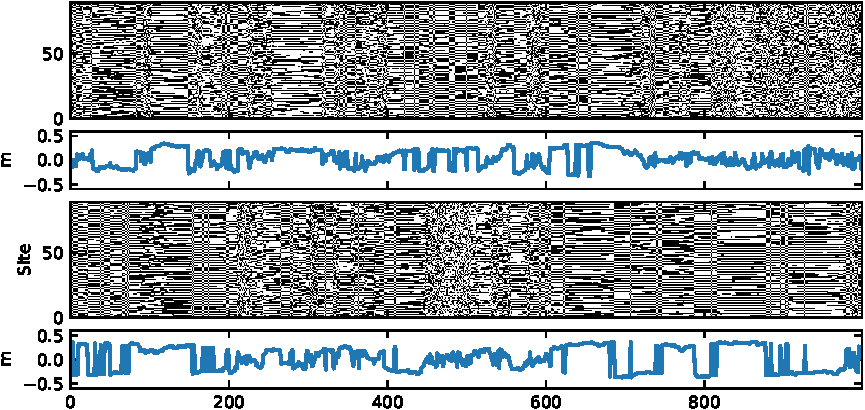
\includegraphics[width=\columnwidth]{pdf_figs/single.pdf}
  \caption{Two MCMC chains starting from the same initial state for a system with $N = 90$ sites and 1000 MCMC steps.  In this simulation the MCMC step is defined differently: an attempt is made to flip n spins, where n is drawn from Uniform(1,N). This is repeated $N^2/100$ times for each step. This trades off computation time for storage space, as it makes the samples less correlated, giving smaller statistical error for a given number of stored samples. These simulations therefore have the potential to necessitate $N^2/100$ matrix diagonalisations for every MCMC sample, though this can be cut down with caching and other tricks. $t = 1, \alpha = 1.25, T = 2.2, J = U = 5 $ \label{fig:single}}
\end{figure}

\%MCMC from an ensemble point of view In implementation \ac{MCMC} can be boiled down to choosing a transition function \$\mathcal{T}(\s\_\{t\} \rightarrow \s\_t+1) \$ where \(\s\) are vectors representing classical spin configurations. We start in some initial state \(\s_0\) and then repeatedly jump to new states according to the probabilities given by \(\mathcal{T}\). This defines a set of random walks \(\{\s_0\ldots \s_i\ldots \s_N\}\). Fig.\textasciitilde{}\ref{fig:single} shows this in practice: we have a (rather small) ensemble of \(M = 2\) walkers starting at the same point in state space and then spreading outwards by flipping spins along the way.

In pseudo-code one could write the MCMC simulation for a single walker as:

\begin{Shaded}
\begin{Highlighting}[]
\NormalTok{current\_state }\OperatorTok{=}\NormalTok{ initial\_state}

\ControlFlowTok{for}\NormalTok{ i }\KeywordTok{in} \BuiltInTok{range}\NormalTok{(N\_steps):}
\NormalTok{    new\_state }\OperatorTok{=}\NormalTok{ sample\_T(current\_state) }
\NormalTok{    states[i] }\OperatorTok{=}\NormalTok{ current\_state}
\end{Highlighting}
\end{Shaded}

Where the \texttt{sample\_T} function here produces a state with probability determined by the \texttt{current\_state} and the transition function \(\mathcal{T}\).

If we ran many such walkers in parallel we could then approximate the distribution \(p_t(\s; \s_0)\) which tells us where the walkers are likely to be after they've evolved for \(t\) steps from an initial state \(\s_0\). We need to carefully choose \(\mathcal{T}\) such that after a large number of steps \(k\) (the convergence time) the probability \(p_t(\s;\s_0)\) approaches the thermal distribution \(P(\s; \beta) = \mathcal{Z}^{-1} e^{-\beta F(\s)}\). This turns out to be quite easy to achieve using the Metropolis-Hasting algorithm.

\hypertarget{convergence-time}{%
\subsubsection{Convergence Time}\label{convergence-time}}

Considering \(p(\s)\) as a vector \(\vec{p}\) whose jth entry is the probability of the jth state \(p_j = p(\s_j)\), and writing \(\mathcal{T}\) as the matrix with entries \(T_{ij} = \mathcal{T}(\s_j \rightarrow \s_i)\) we can write the update rule for the ensemble probability as: \[\vec{p}_{t+1} = \mathcal{T} \vec{p}_t \implies \vec{p}_{t} = \mathcal{T}^t \vec{p}_0\] where \(\vec{p}_0\) is vector which is one on the starting state and zero everywhere else. Since all states must transition to somewhere with probability one: \(\sum_i T_{ij} = 1\).

Matrices that satisfy this are called stochastic matrices exactly because they model these kinds of Markov processes. It can be shown that they have real eigenvalues, and ordering them by magnitude, that \(\lambda_0 = 1\) and \(0 < \lambda_{i\neq0} < 1\). \%https://en.wikipedia.org/wiki/Stochastic\_matrix

Assuming \(\mathcal{T}\) has been chosen correctly, its single eigenvector with eigenvalue 1 will be the thermal distribution \footnote{or, in the general case, any desired distribution. MCMC has found a lot of use in sampling from the complicated distributions that arise when taking a Bayesian approach to statistics.} so repeated application of the transition function eventually leads there, while memory of the initial conditions decays exponentially with a convergence time \(k\) determined by \(\lambda_1\). In practice this means that one throws away the data from the beginning of the random walk in order reduce the dependence on the initial conditions and be close enough to the target distribution.

\hypertarget{auto-correlation-time}{%
\subsubsection{Auto-correlation Time}\label{auto-correlation-time}}

\begin{figure}
\hypertarget{fig:m_autocorr}{%
\centering
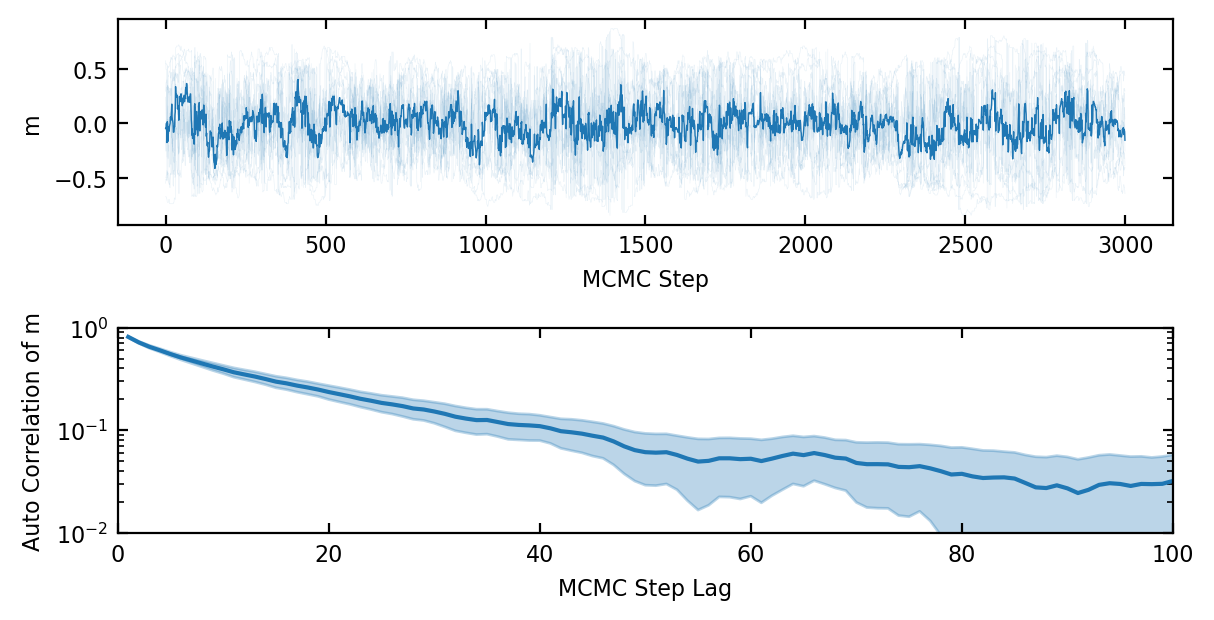
\includegraphics[width=1\textwidth,height=\textheight]{figure_code/fk_chapter/lsr/figs/m_autocorr.png}
\caption[no title]{(Upper) 10 MCMC chains starting from the same initial state for
a system with \(N = 150\) sites and 3000 MCMC steps. At each MCMC step,
n spins are flipped where n is drawn from Uniform(1,N) and this is
repeated \(N^2/100\) times. The simulations therefore have the potential
to necessitate \(10*N^2\) matrix diagonalisations for each 100 MCMC
steps. (Lower) The normalised auto-correlation
\((\expval{m_i m_{i-j}} - \expval{m_i}\expval{m_i}) / Var(m_i))\)
averaged over \(i\). It can be seen that even with each MCMC step
already being composed of many individual flip attempts, the
auto-correlation is still non negligible and must be taken into account
in the statistics.
\(t = 1, \alpha = 1.25, T = 2.2, J = U = 5\)}\label{fig:m_autocorr}
}
\end{figure}

At this stage one might think we're done. We can indeed draw independent samples from \(P(\s; \beta)\) by starting from some arbitrary initial state and doing \(k\) steps to arrive at a sample. However a key insight is that after the convergence time, every state generated is a sample from \(P(\s; \beta)\)! They are not, however, independent samples. In Fig.\textasciitilde{}\ref{fig:raw} it is already clear that the samples of the order parameter m have some auto-correlation because only a few spins are flipped each step but even when the number of spins flipped per step is increased, Fig.\textasciitilde{}\ref{fig:m_autocorr} shows that it can be an important effect near the phase transition. Let's define the auto-correlation time \(\tau(O)\) informally as the number of MCMC samples of some observable O that are statistically equal to one independent sample or equivalently as the number of MCMC steps after which the samples are correlated below some cutoff, see \autocite{krauthIntroductionMonteCarlo1996} for a more rigorous definition involving a sum over the auto-correlation function. The auto-correlation time is generally shorter than the convergence time so it therefore makes sense from an efficiency standpoint to run a single walker for many MCMC steps rather than to run a huge ensemble for \(k\) steps each.

Once the random walk has been carried out for many steps, the expectation values of \(O\) can be estimated from the MCMC samples \(\s_i\): \[
    \tex{O} = \sum_{i = 0}^{N} O(\s_i) + \mathcal{O}(\frac{1}{\sqrt{N}})
\] The the samples are correlated so the N of them effectively contains less information than \(N\) independent samples would, in fact roughly \(N/\tau\) effective samples. As a consequence the variance is larger than the \(\qex{O^2} - \qex{O}^2\) form it would have if the estimates were uncorrelated. There are many methods in the literature for estimating the true variance of \(\qex{O}\) and deciding how many steps are needed but my approach has been to run a small number of parallel chains, which are independent, in order to estimate the statistical error produced. This is a slightly less computationally efficient because it requires throwing away those \(k\) steps generated before convergence multiple times but it is a conceptually simple workaround.

In summary, to do efficient simulations we want to reduce both the convergence time and the auto-correlation time as much as possible. In order to explain how, we need to introduce the Metropolis-Hasting (MH) algorithm and how it gives an explicit form for the transition function.

\hypertarget{the-metropolis-hastings-algorithm}{%
\subsubsection{The Metropolis-Hastings Algorithm}\label{the-metropolis-hastings-algorithm}}

MH breaks up the transition function into a proposal distribution \(q(\s \to \s')\) and an acceptance function \(\mathcal{A}(\s \to \s')\). \(q\) needs to be something that we can directly sample from, and in our case generally takes the form of flipping some number of spins in \(\s\), i.e if we're flipping a single random spin in the spin chain, \(q(\s \to \s')\) is the uniform distribution on states reachable by one spin flip from \(\s\). This also gives the nice symmetry property that \(q(\s \to \s') = q(\s' \to \s)\).

The proposal \(\s'\) is then accepted or rejected with an acceptance probability \(\mathcal{A}(\s \to \s')\), if the proposal is rejected then \(\s_{i+1} = \s_{i}\). Hence:

\[\mathcal{T}(x\to x') = q(x\to x')\mathcal{A}(x \to x')\]

When the proposal distribution is symmetric as ours is, it cancels out in the expression for the acceptance function and the Metropolis-Hastings algorithm is simply the choice: \[ \mathcal{A}(x \to x') = \min\left(1, e^{-\beta\;\Delta F}\right)\] Where \(F\) is the overall free energy of the system, including both the quantum and classical sector.

To implement the acceptance function in practice we pick a random number in the unit interval and accept if it is less than \(e^{-\beta\;\Delta F}\):

\begin{Shaded}
\begin{Highlighting}[]
\NormalTok{current\_state }\OperatorTok{=}\NormalTok{ initial\_state}

\ControlFlowTok{for}\NormalTok{ i }\KeywordTok{in} \BuiltInTok{range}\NormalTok{(N\_steps):}
\NormalTok{    new\_state }\OperatorTok{=}\NormalTok{ proposal(current\_state)}
\NormalTok{    df }\OperatorTok{=}\NormalTok{ free\_energy\_change(current\_state, new\_state, parameters)}

    \ControlFlowTok{if}\NormalTok{ uniform(}\DecValTok{0}\NormalTok{,}\DecValTok{1}\NormalTok{) }\OperatorTok{\textless{}}\NormalTok{ exp(}\OperatorTok{{-}}\NormalTok{beta }\OperatorTok{*}\NormalTok{ df):}
\NormalTok{        current\_state }\OperatorTok{=}\NormalTok{ new\_state}
        
\NormalTok{    states[i] }\OperatorTok{=}\NormalTok{ current\_state}
\end{Highlighting}
\end{Shaded}

This has the effect of always accepting proposed states that are lower in energy and sometimes accepting those that are higher in energy than the current state.

\hypertarget{two-step-trick}{%
\subsection{Two Step Trick}\label{two-step-trick}}

Here, we incorporate a modification to the standard Metropolis-Hastings algorithm~\autocite{hastingsMonteCarloSampling1970} gleaned from Krauth~\autocite{krauthIntroductionMonteCarlo1998}.

In our computations~\autocite{hodsonMCMCFKModel2021} we employ a modification of the algorithm which is based on the observation that the free energy of the FK system is composed of a classical part which is much quicker to compute than the quantum part. Hence, we can obtain a computational speedup by first considering the value of the classical energy difference \(\Delta H_s\) and rejecting the transition if the former is too high. We only compute the quantum energy difference \(\Delta F_c\) if the transition is accepted. We then perform a second rejection sampling step based upon it. This corresponds to two nested comparisons with the majority of the work only occurring if the first test passes and has the acceptance function \[\mathcal{A}(a \to b) = \min\left(1, e^{-\beta \Delta H_s}\right)\min\left(1, e^{-\beta \Delta F_c}\right)\;.\]

For the model parameters used in Fig.~\protect\hyperlink{fig:indiv_IPR}{2}, we find that with our new scheme the matrix diagonalisation is skipped around 30\% of the time at \(T = 2.5\) and up to 80\% at \(T = 1.5\). We observe that for \(N = 50\), the matrix diagonalisation, if it occurs, occupies around 60\% of the total computation time for a single step. This rises to 90\% at N = 300 and further increases for larger N. We therefore get the greatest speedup for large system sizes at low temperature where many prospective transitions are rejected at the classical stage and the matrix computation takes up the greatest fraction of the total computation time. The upshot is that we find a speedup of up to a factor of 10 at the cost of very little extra algorithmic complexity.

Our two-step method should be distinguished from the more common method for speeding up MCMC which is to add asymmetry to the proposal distribution to make it as similar as possible to \(\min\left(1, e^{-\beta \Delta E}\right)\). This reduces the number of rejected states, which brings the algorithm closer in efficiency to a direct sampling method. However it comes at the expense of requiring a way to directly sample from this complex distribution, a problem which MCMC was employed to solve in the first place. For example, recent work trains restricted Boltzmann machines (RBMs) to generate samples for the proposal distribution of the FK model~\autocite{huangAcceleratedMonteCarlo2017}. The RBMs are chosen as a parametrisation of the proposal distribution that can be efficiently sampled from while offering sufficient flexibility that they can be adjusted to match the target distribution. Our proposed method is considerably simpler and does not require training while still reaping some of the benefits of reduced computation.

\hypertarget{detailed-balance-for-the-two-step-method}{%
\subsection{Detailed Balance for the two step method}\label{detailed-balance-for-the-two-step-method}}

Given a MCMC algorithm with target distribution \(\pi(a)\) and transition function \(\mathcal{T}\) the detailed balance condition is sufficient (along with some technical constraints \autocite{wolffMonteCarloErrors2004}) to guarantee that in the long time limit the algorithm produces samples from \(\pi\). \[\pi(a)\mathcal{T}(a \to b) = \pi(b)\mathcal{T}(b \to a)\]

In pseudo-code, our two step method corresponds to two nested comparisons with the majority of the work only occurring if the first test passes:

\begin{Shaded}
\begin{Highlighting}[]
\NormalTok{current\_state }\OperatorTok{=}\NormalTok{ initial\_state}

\ControlFlowTok{for}\NormalTok{ i }\KeywordTok{in} \BuiltInTok{range}\NormalTok{(N\_steps):}
\NormalTok{  new\_state }\OperatorTok{=}\NormalTok{ proposal(current\_state)}

\NormalTok{  c\_dE }\OperatorTok{=}\NormalTok{ classical\_energy\_change(}
\NormalTok{                               current\_state,}
\NormalTok{                               new\_state)}
  \ControlFlowTok{if}\NormalTok{ uniform(}\DecValTok{0}\NormalTok{,}\DecValTok{1}\NormalTok{) }\OperatorTok{\textless{}}\NormalTok{ exp(}\OperatorTok{{-}}\NormalTok{beta }\OperatorTok{*}\NormalTok{ c\_dE):}
\NormalTok{    q\_dF }\OperatorTok{=}\NormalTok{ quantum\_free\_energy\_change(}
\NormalTok{                                current\_state,}
\NormalTok{                                new\_state)}
    \ControlFlowTok{if}\NormalTok{ uniform(}\DecValTok{0}\NormalTok{,}\DecValTok{1}\NormalTok{) }\OperatorTok{\textless{}}\NormalTok{ exp(}\OperatorTok{{-}}\NormalTok{ beta }\OperatorTok{*}\NormalTok{ q\_dF):}
\NormalTok{      current\_state }\OperatorTok{=}\NormalTok{ new\_state}

\NormalTok{    states[i] }\OperatorTok{=}\NormalTok{ current\_state}
\end{Highlighting}
\end{Shaded}

Defining \(r_c = e^{-\beta H_c}\) and \(r_q = e^{-\beta F_q}\) our target distribution is \(\pi(a) = r_c r_q\). This method has \(\mathcal{T}(a\to b) = q(a\to b)\mathcal{A}(a \to b)\) with symmetric \(p(a \to b) = \pi(b \to a)\) and \(\mathcal{A} = \min\left(1, r_c\right) \min\left(1, r_q\right)\)

Substituting this into the detailed balance equation gives: \[\mathcal{T}(a \to b)/\mathcal{T}(b \to a) = \pi(b)/\pi(a) = r_c r_q\]

Taking the LHS and substituting in our transition function: \[\begin{aligned}
\mathcal{T}(a \to b)/\mathcal{T}(b \to a) = \frac{\min\left(1, r_c\right) \min\left(1, r_q\right)}{ \min\left(1, 1/r_c\right) \min\left(1, 1/r_q\right)}\end{aligned}\]

which simplifies to \(r_c r_q\) as \(\min(1,r)/\min(1,1/r) = r\) for \(r > 0\).

\hypertarget{two-step-trick-1}{%
\subsubsection{Two Step Trick}\label{two-step-trick-1}}

Our method already relies heavily on the split between the classical and quantum sector to derive a sign problem free MCMC algorithm but it turns out that there is a further trick we can play with it. The free energy term is the sum of an easy to compute classical energy and a more expensive quantum free energy, we can split the acceptance function into two in such as way as to avoid having to compute the full exact diagonalisation some of the time:

\begin{Shaded}
\begin{Highlighting}[]

\NormalTok{current\_state }\OperatorTok{=}\NormalTok{ initial\_state}

\ControlFlowTok{for}\NormalTok{ i }\KeywordTok{in} \BuiltInTok{range}\NormalTok{(N\_steps):}
\NormalTok{    new\_state }\OperatorTok{=}\NormalTok{ proposal(current\_state)}

\NormalTok{    df\_classical }\OperatorTok{=}\NormalTok{ classical\_free\_energy\_change(current\_state, new\_state, parameters)}
    \ControlFlowTok{if}\NormalTok{ exp(}\OperatorTok{{-}}\NormalTok{beta }\OperatorTok{*}\NormalTok{ df\_classical) }\OperatorTok{\textless{}}\NormalTok{ uniform(}\DecValTok{0}\NormalTok{,}\DecValTok{1}\NormalTok{):}
\NormalTok{        f\_quantum }\OperatorTok{=}\NormalTok{ quantum\_free\_energy(current\_state, new\_state, parameters)}
    
        \ControlFlowTok{if}\NormalTok{ exp(}\OperatorTok{{-}}\NormalTok{ beta }\OperatorTok{*}\NormalTok{ df\_quantum) }\OperatorTok{\textless{}}\NormalTok{ uniform(}\DecValTok{0}\NormalTok{,}\DecValTok{1}\NormalTok{):}
\NormalTok{          current\_state }\OperatorTok{=}\NormalTok{ new\_state}
    
\NormalTok{        states[i] }\OperatorTok{=}\NormalTok{ current\_state}
    
\end{Highlighting}
\end{Shaded}

\hypertarget{tuning-the-proposal-distribution}{%
\subsubsection{Tuning the proposal distribution}\label{tuning-the-proposal-distribution}}

\begin{figure}
\hypertarget{fig:autocorr_multiple_proposals}{%
\centering
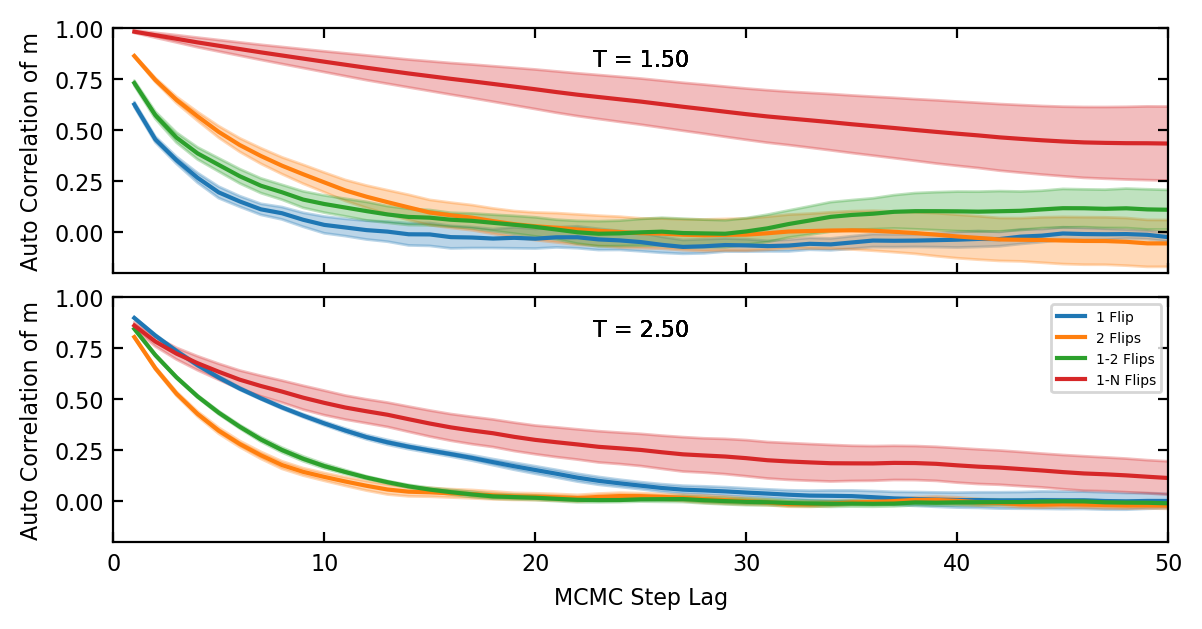
\includegraphics[width=1\textwidth,height=\textheight]{figure_code/fk_chapter/lsr/figs/autocorr_multiple_proposals.png}
\caption[no title]{Simulations showing how the autocorrelation of the order
parameter depends on the proposal distribution used at different
temperatures, we see that at \(T = 1.5 < T_c\) a single spin flip is
likely the best choice, while at the high temperature \(T = 2.5 > T_c\)
flipping two sites or a mixture of flipping two and 1 sites is likely a
better choice. \$t = 1, \alpha = 1.25, J = U = 5
\$}\label{fig:autocorr_multiple_proposals}
}
\end{figure}

Now we can discuss how to minimise the auto-correlations. The general principle is that one must balance the proposal distribution between two extremes. Choose overlay small steps, like flipping only a single spin and the acceptance rate will be high because \(\Delta F\) will usually be small, but each state will be very similar to the previous and the auto-correlations will be high too, making sampling inefficient. On the other hand, overlay large steps, like randomising a large portion of the spins each step, will result in very frequent rejections, especially at low temperatures.

I evaluated a few different proposal distributions for use with the FK model.

\begin{enumerate}
\def\labelenumi{\arabic{enumi}.}
\tightlist
\item
  Flipping a single random site
\item
  Flipping N random sites for some N
\item
  Choosing n from Uniform(1, N) and then flipping n sites for some fixed N.
\item
  Attempting to tune the proposal distribution for each parameter regime.
\end{enumerate}

Fro Figure\textasciitilde{}\ref{fig:comparison} we see that even at moderately high temperatures \(T > T_c\) flipping one or two sites is the best choice. However for some simulations at very high temperature flipping more spins is warranted. Tuning the proposal distribution automatically seems like something that would not yield enough benefit for the additional complexity it would require.

\hypertarget{diagnostics-of-localisation}{%
\section{Diagnostics of Localisation}\label{diagnostics-of-localisation}}

\hypertarget{inverse-participation-ratio}{%
\subsection{Inverse Participation Ratio}\label{inverse-participation-ratio}}

The inverse participation ratio is defined for a normalised wave function \(\psi_i = \psi(x_i), \sum_i \abs{\psi_i}^2 = 1\) as its fourth moment \autocite{kramerLocalizationTheoryExperiment1993}: \[
P^{-1} = \sum_i \abs{\psi_i}^4
\] \% It acts as a measure of the portion of space occupied by the wave function. For localised states it will be independent of system size while for plane wave states in d dimensions \$P = L\^{}d \$. States may also be intermediate between localised and extended, described by their fractal dimensionality \(d > d* > 0\): \[
P(L) \goeslike L^{d*} 
\] \% For extended states \(d* = 0\) while for localised ones \(d* = 0\). In this work we take use an energy resolved IPR \autocite{andersonAbsenceDiffusionCertain1958}: \[
DOS(\omega) = \sum_n \delta(\omega - \epsilon_n)
IPR(\omega) = DOS(\omega)^{-1} \sum_{n,i} \delta(\omega - \epsilon_n) \abs{\psi_{n,i}}^4
\] Where \(\psi_{n,i}\) is the wavefunction corresponding to the energy \(\epsilon_n\) at the ith site. In practice we bin the energies and IPRs into a fine energy grid and use Lorentzian smoothing if necessary.

\begin{Shaded}
\begin{Highlighting}[]

\end{Highlighting}
\end{Shaded}
